\chapter{Results and Discussion} \label{chp:4}

Analysis of the results were done via respective normalization and visualization methods. A two step normalization was achieved through the use of a Gaussian smoothing kernel ($\frac{1}{\sqrt{2\pi}}e^{-\frac{u^2}{2}}$) and probability density function ($\frac{1}{nh}\sum^n_{i=1}K(\frac{x-x_i}{h})$). The smoothing kernel treats each point in the data as an individual, contributing to the overall density of the whole. This is done by expanding it to a normal distribution, with $x$ and $y$ coordinates representing the respective means. Applying this smoothing function to each point in the data set, one is able to achieve a collection of normal distributions that can be summed in order relate all points to one another in the distribution space. This collective distribution is normalized via a probability density function which has the inherent property of leaving the entire area under the curve as equal to one. Therefore each respective range in question represents a part of this unity. From this a graph is generated, indicating the density distribution of the underlying data as shown by figure \ref{TwoResPDF}.

A second step towards understanding the data involved the use of three neural networks, separately trained on $80\%$ of the data and validated against the remaining $20\%$. From these trained models, one is able to make predictions on flux control co\"efficent based on the disequilibrium ratio values. The accuracy of the prediction of control coe are based on the underlying data and as such a probability distribution of such a prediction, describes the confidence level of the predictive function. This can be seen in figure \ref{PredictionConfidence}, where a standard deviation, or confidence interval, of the predicted value is reliant upon the disequilibrium ratio in question. 

From data processing, transformation and visualisation the logical ordering of operations followed are akin to that of a data-flow paradigm. With individual functions serving as static nodes to data, whereas inside of the functions a control flow paradigm is utilised with functions being applied to the data itself. This hybrid data/control flow proved useful in maintaining accuracy as brought by control-flow, alongside the speed gains that the parallelism of a data-flow paradigm yields. These methods of this investigation, as described in chapter \ref{chp:3}, lead to the generation of log files that were visualized in a directed graph form. This graph, figure \ref{Graph_modDistro}, indicates the flow of model information throughout the algorithm run time. 

\begin{figure}[p] 
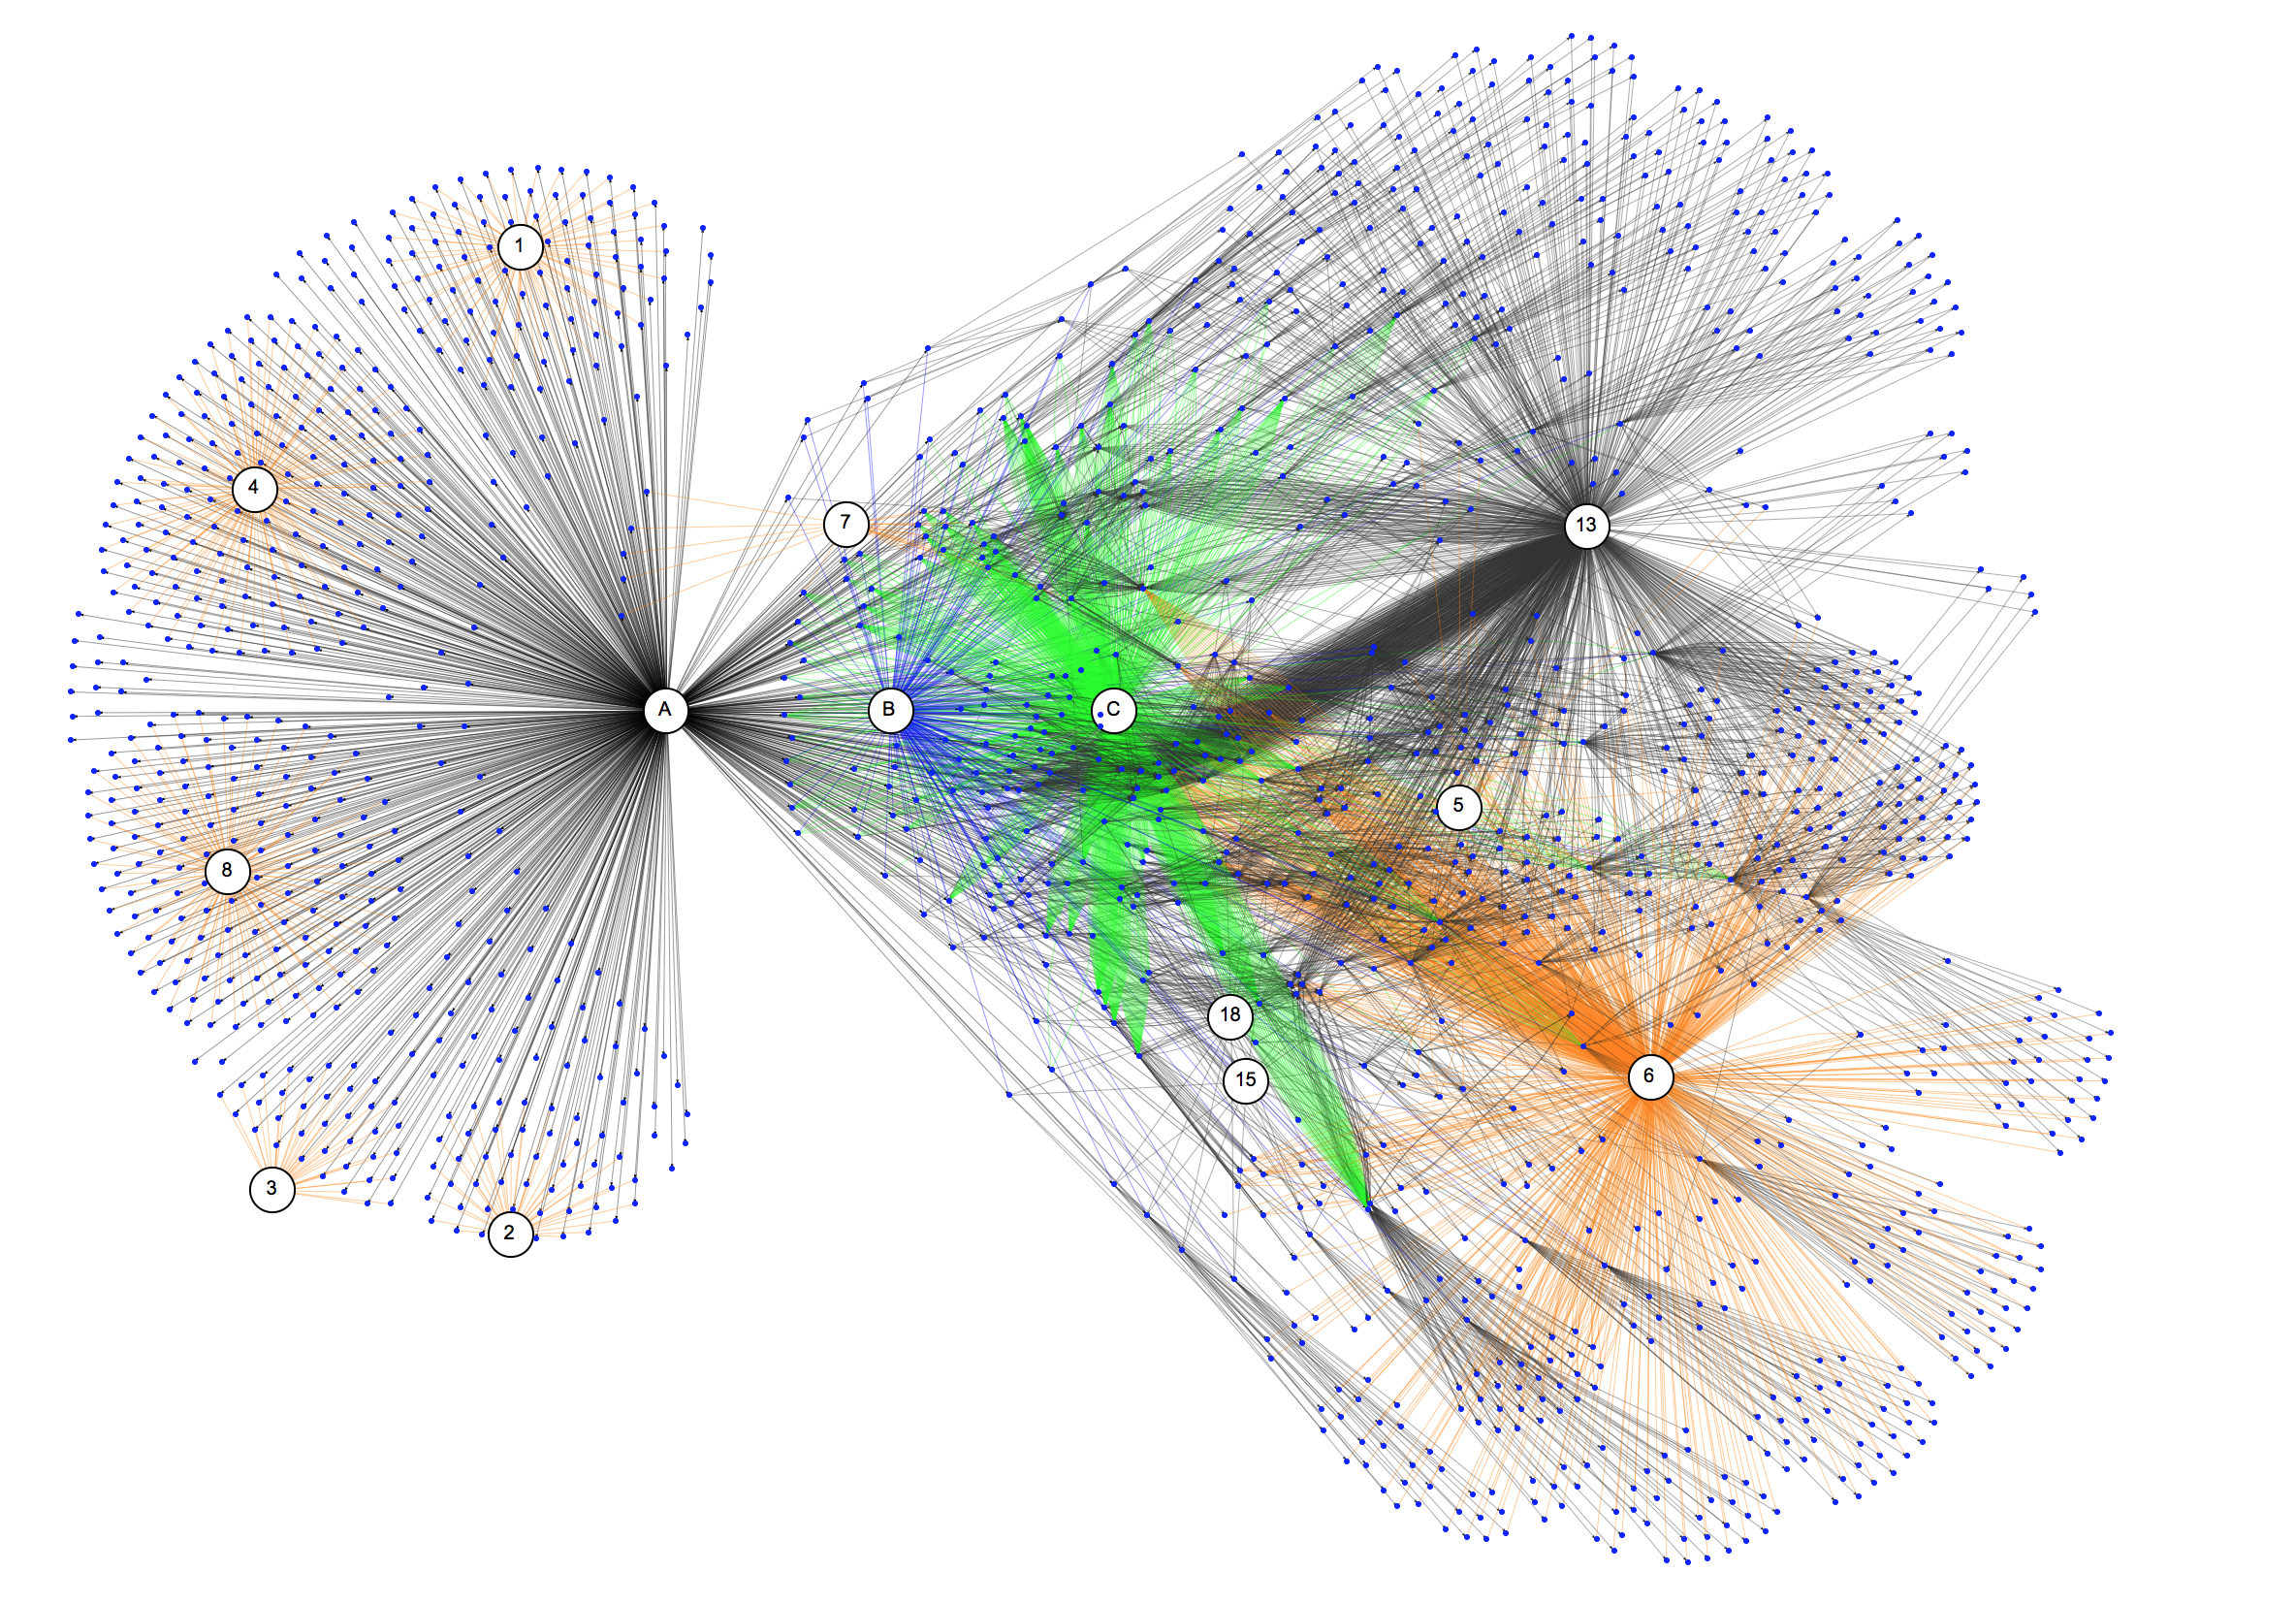
\includegraphics[width=1\textwidth]{figs/Digraph.png}
\centering
\caption{A directed graph indicating the flow of models as they are filtered by the algorithm described in chapter \ref{chp:3}. 
Important checkpoints are indicated by letters, with $A \rightarrow{}$ All models, $B \rightarrow{}$ Has reversible rates and $C \rightarrow{}$ Initial check functions passed. Filter criteria is labeled by number, with $1 \rightarrow{}$ No stoichiometries, $2 \rightarrow{}$ Models containing events, $3 \rightarrow{}$ Piece-wise funcitons in model, $4 \rightarrow{}$ Oscillatory Behaviour, $5 \rightarrow{}$ Errors in division by zero, $6 \rightarrow{}$ Flux summation errors, $7 \rightarrow{}$ Models timed out, $8 \rightarrow{}$ No reversible reactions, $9 \rightarrow{}$ Import error, $10 \rightarrow{}$ Negative FCC, $11 \rightarrow{}$ Steady-state error, $12 \rightarrow{}$ Division by zero, $13 \rightarrow{}$ No product or substrate, $14 \rightarrow{}$ Replacement errors, $15 \rightarrow{}$ Small maximum elasticity coefficient, $16 \rightarrow{}$ No reversible reactions, $17 \rightarrow{}$ Flux calculation error and $18 \rightarrow{}$ No flux results generated.}
\label{Graph_modDistro}
\end{figure}

This figure allows one to gain an overview of the model space. The models of importance were ones leading towards $C$ with green lines, it is however clear that many models did not meet the requirements. The final data contains reactions from 111 models, yielding 843 reversible reaction points on disequilibrium ratio and flux control co\"efficient.

A probability density function of the distribution, normalized by a Gaussian (normal) kernel, was visualized by a contour plot. This plot can be seen at two resolutions in figure \ref{TwoResPDF}. It is clear that there exists a tendency for reactions close to equilibrium to not have a large degree of own flux control. This can be seen from figure \ref{TwoResPDF} $a$, where there is no representative reaction with a control co\"eficient larger than $0.4$. On the opposite side of the scale it is observed that reactions with a larger than $0.4$ control co\"efficient, reside within the region of $\rho < 0.1$. The $\rho$ separation values chosen above can be seen in figure \ref{LitCompare}. These values echo the conclusion by \citeauthor{Rohwer2009} as discussed in chapter \ref{chp:2}. At a higher resolution, figure \ref{TwoResPDF} $b$ indicates that reactions close to equilibrium ($\rho > 0.8$), with larger than $0.4$ flux control co\"efficients do exist. 

\begin{figure}[p] \label{TwoResPDF}
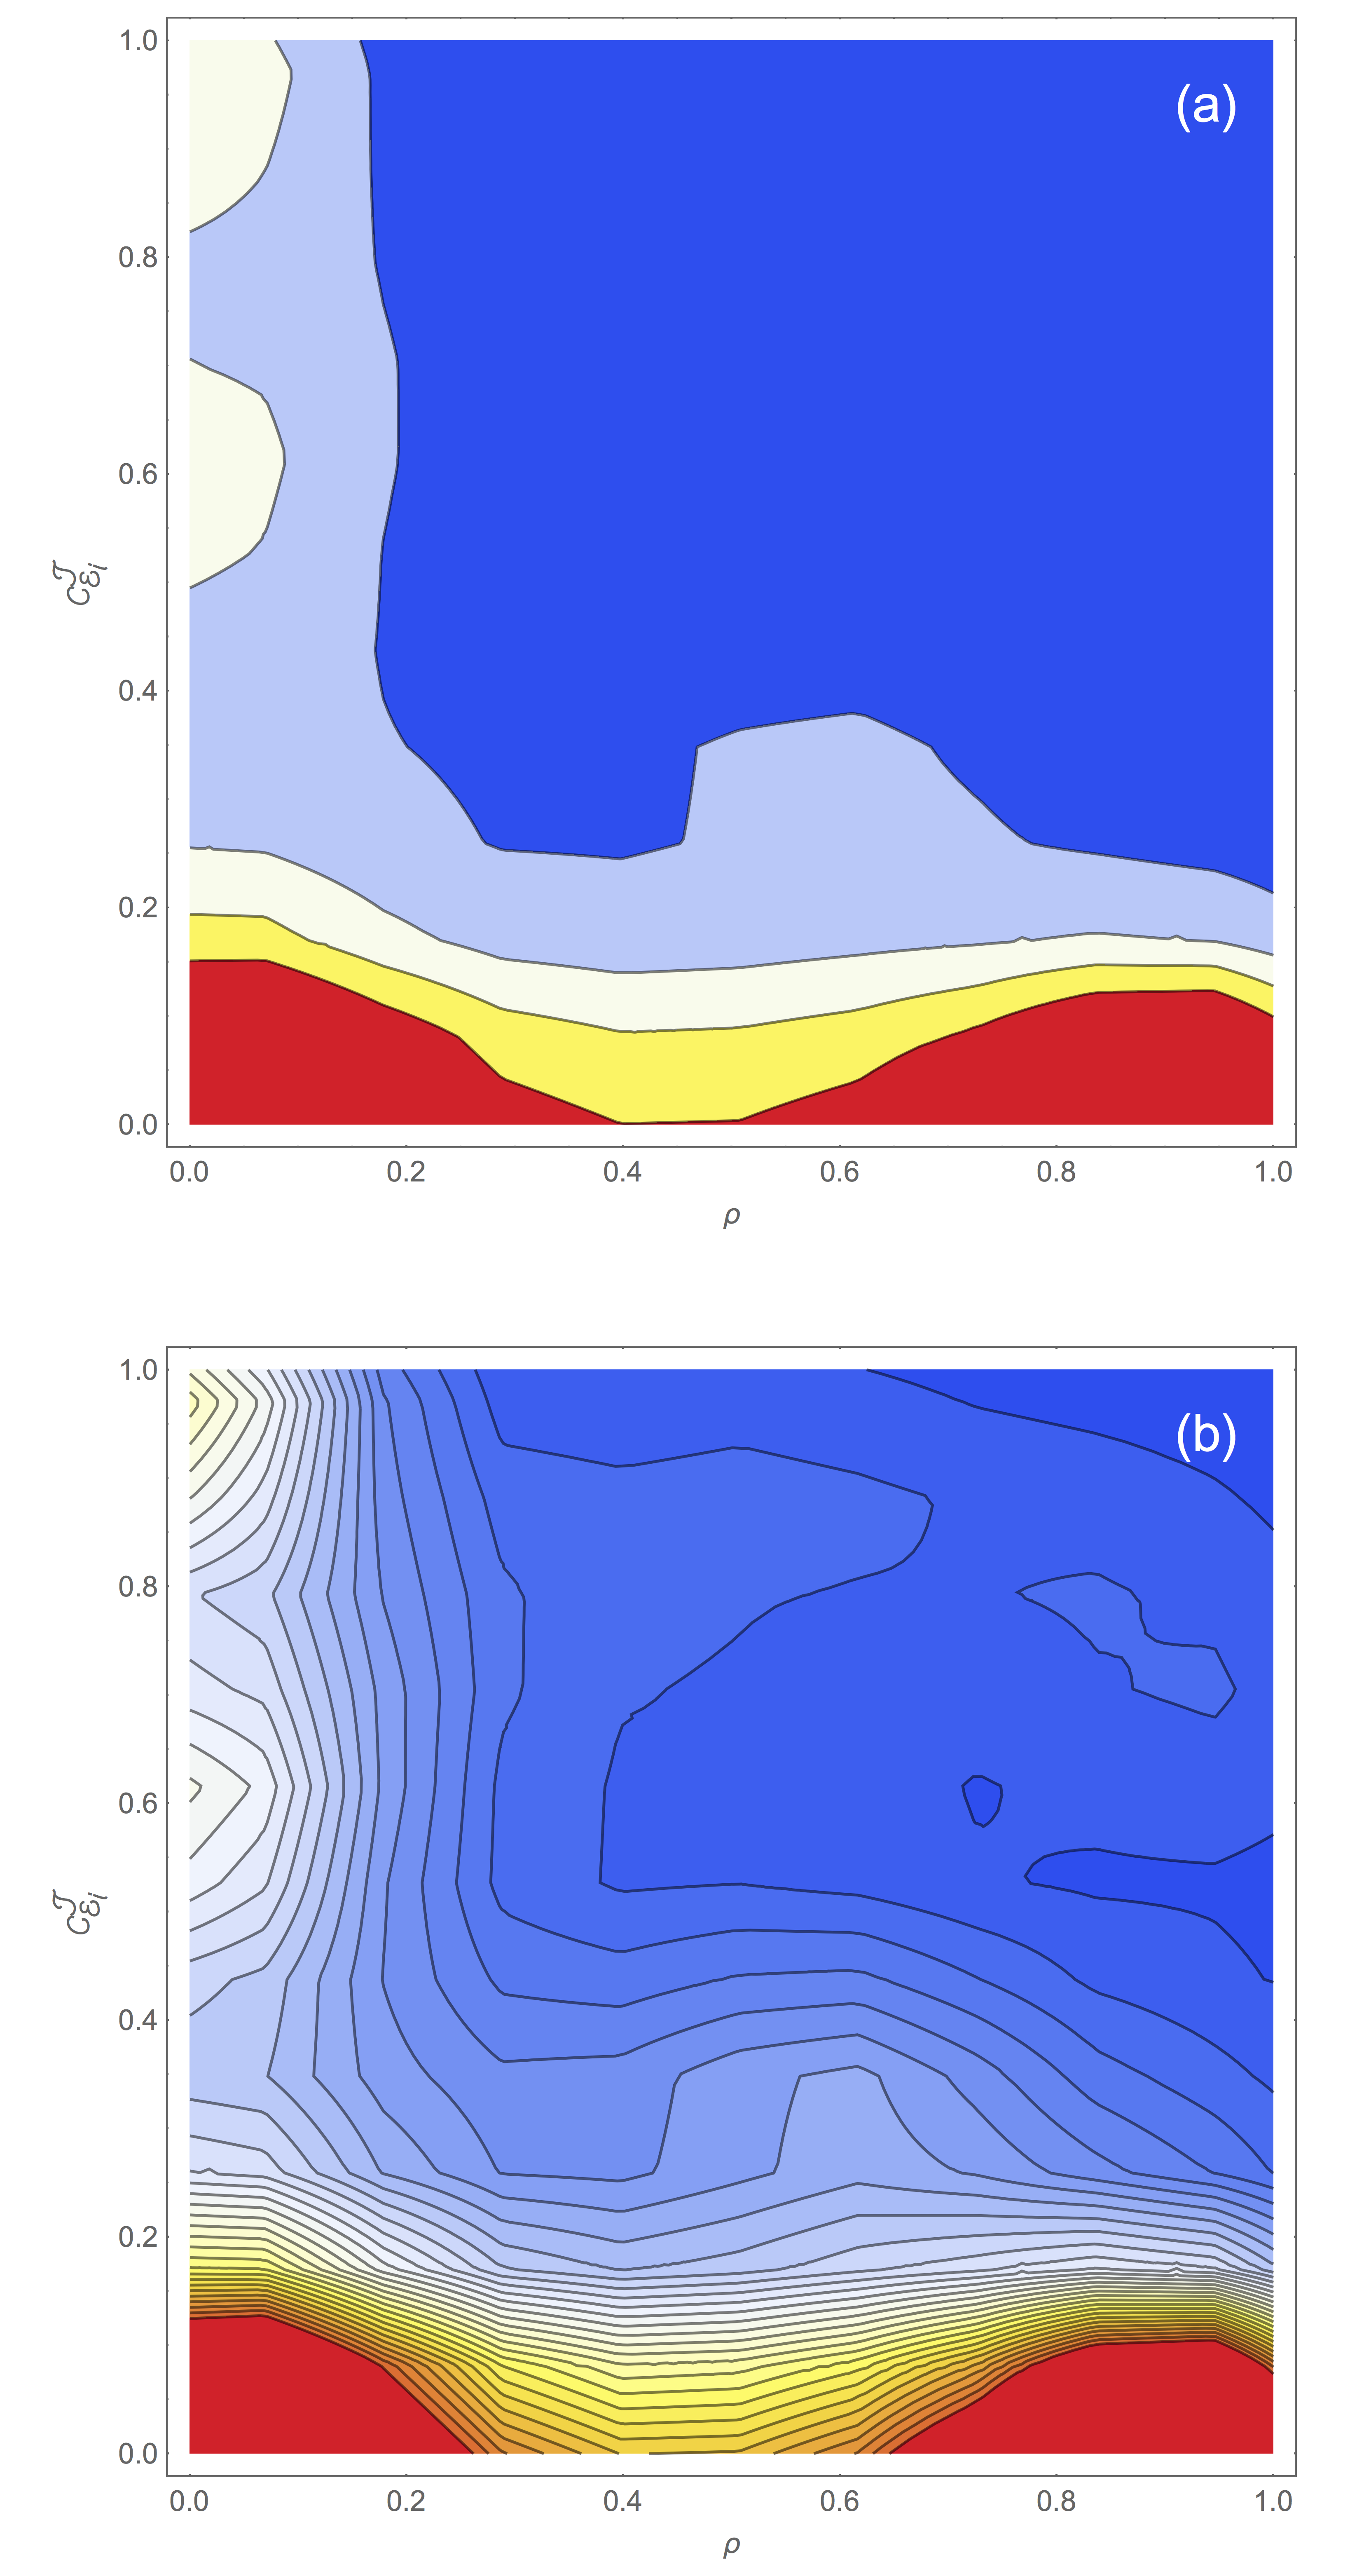
\includegraphics[width=0.8\textwidth]{figs/TwoResPDF.png}
\centering
\caption{Two resolutions was obtained by varying the contour amount visualized, $a = 4$ and $b = 30$, from the probability density function calculated in chapter \ref{chp:3}. This data is on the disequilibrium ratio ($\rho$) and the own flux control coefficient ($C_{E_i}^J$), normalized to the probability space of one. Red and blue respectively denote high and low density areas of data points.}
\end{figure}

\begin{figure}[p] 
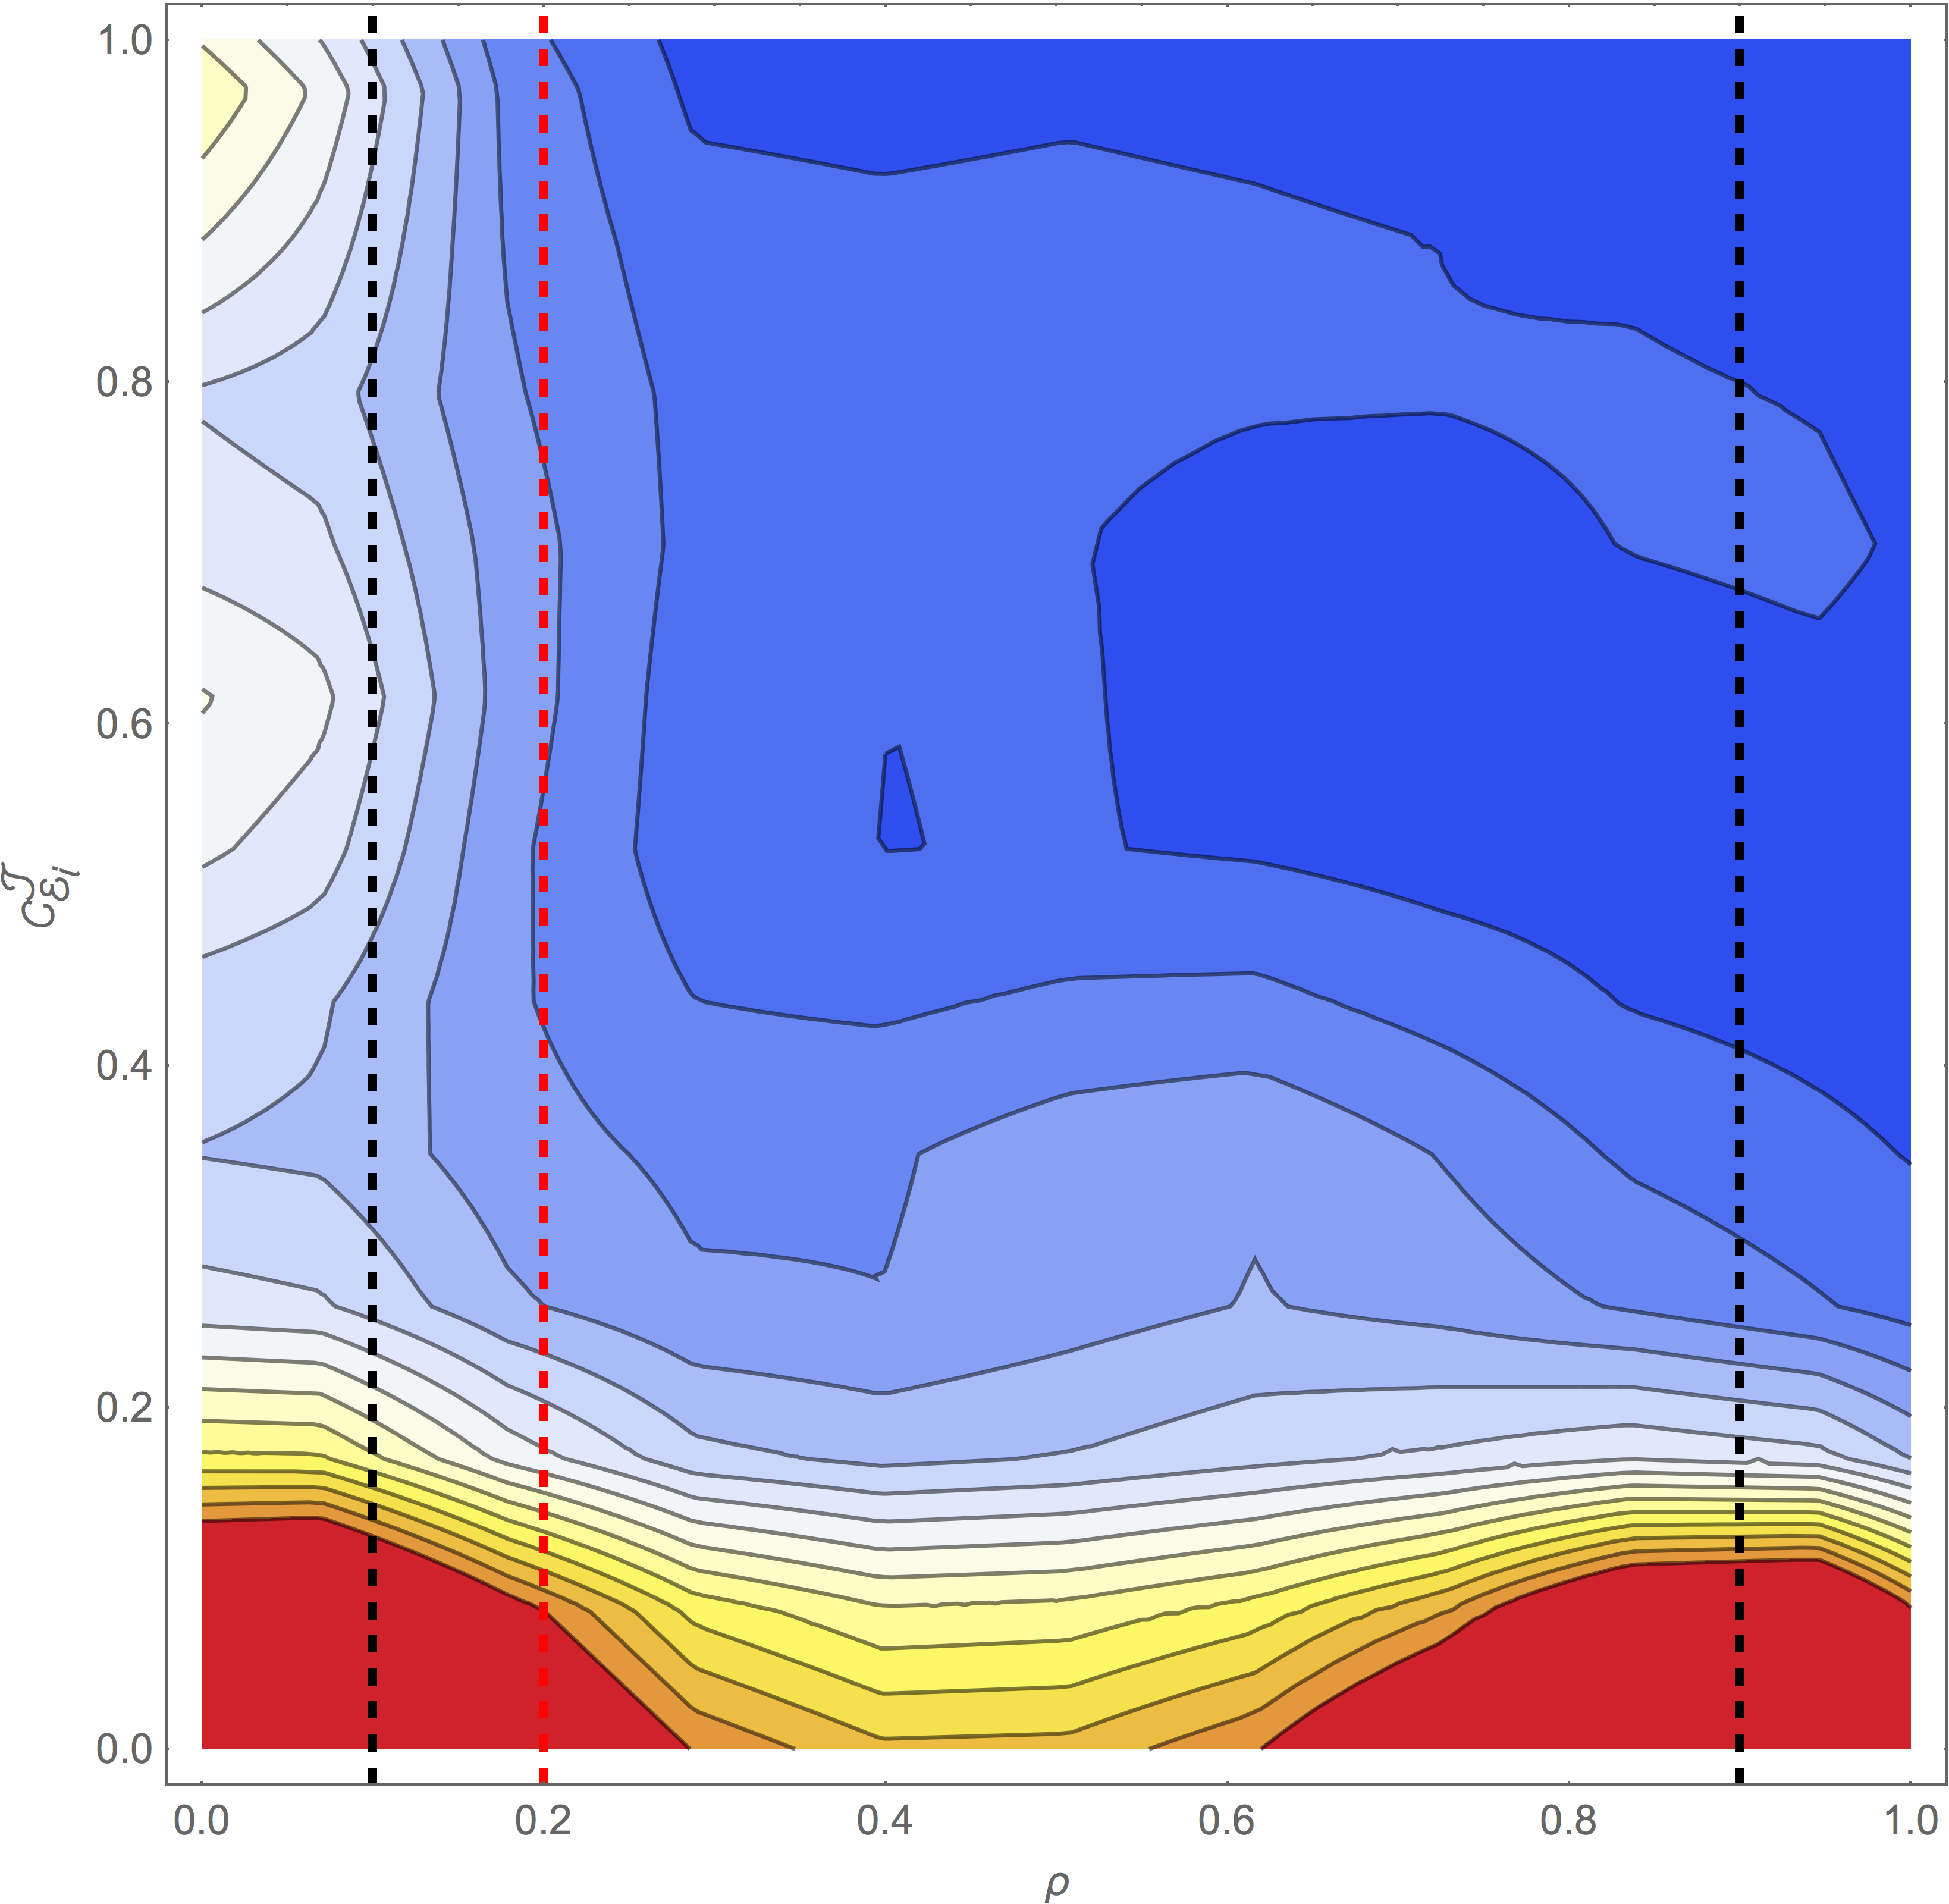
\includegraphics[width=0.8\textwidth]{figs/LitCompare.png} \label{LitCompare}
\centering
\caption{Probability density function of data gathered. This data is on the disequilibrium ratio ($\rho$) and the own flux control coefficient ($C_{E_i}^J$), normalized to the probability space of 1. Red and blue respectively denote high and low density areas of data points. The black (\citeauthor{Rohwer2009}) and red (\citeauthor{ROLLESTON1972}) dashed lines indicate respective authors views, as referred to in chapter \ref{chp:2}, on probable conditions of dominating contributions to regulation.}
\end{figure}

To gain a quantitative degree of confidence in the visual findings, the data was used as input in the training of three separate neural networks, described in \ref{chp:3}. The probability density functions of the returned predictions on flux control co\"efficients were visualized on a single axes in figure \ref{PredConf}. It can be seen that all three networks produce similar confidence intervals, where reactions close to equilibrium ($d$ and $e$) have a low probability of yielding a reaction with a high flux control co\"efficient. Conversely, reactions at disequilibrium ratios far from equilibrium ($a$ to $c$) yields a larger degree of likely hood that said reaction will have a high self flux control co\"efficient. A third condition is observed in figure \ref{PredictionConfidence} where reactions far from equilibrium ($a$ to $c$) have low flux control co\"efficients ($C_{E_i}^J <0.2$) .

\begin{figure}[p]
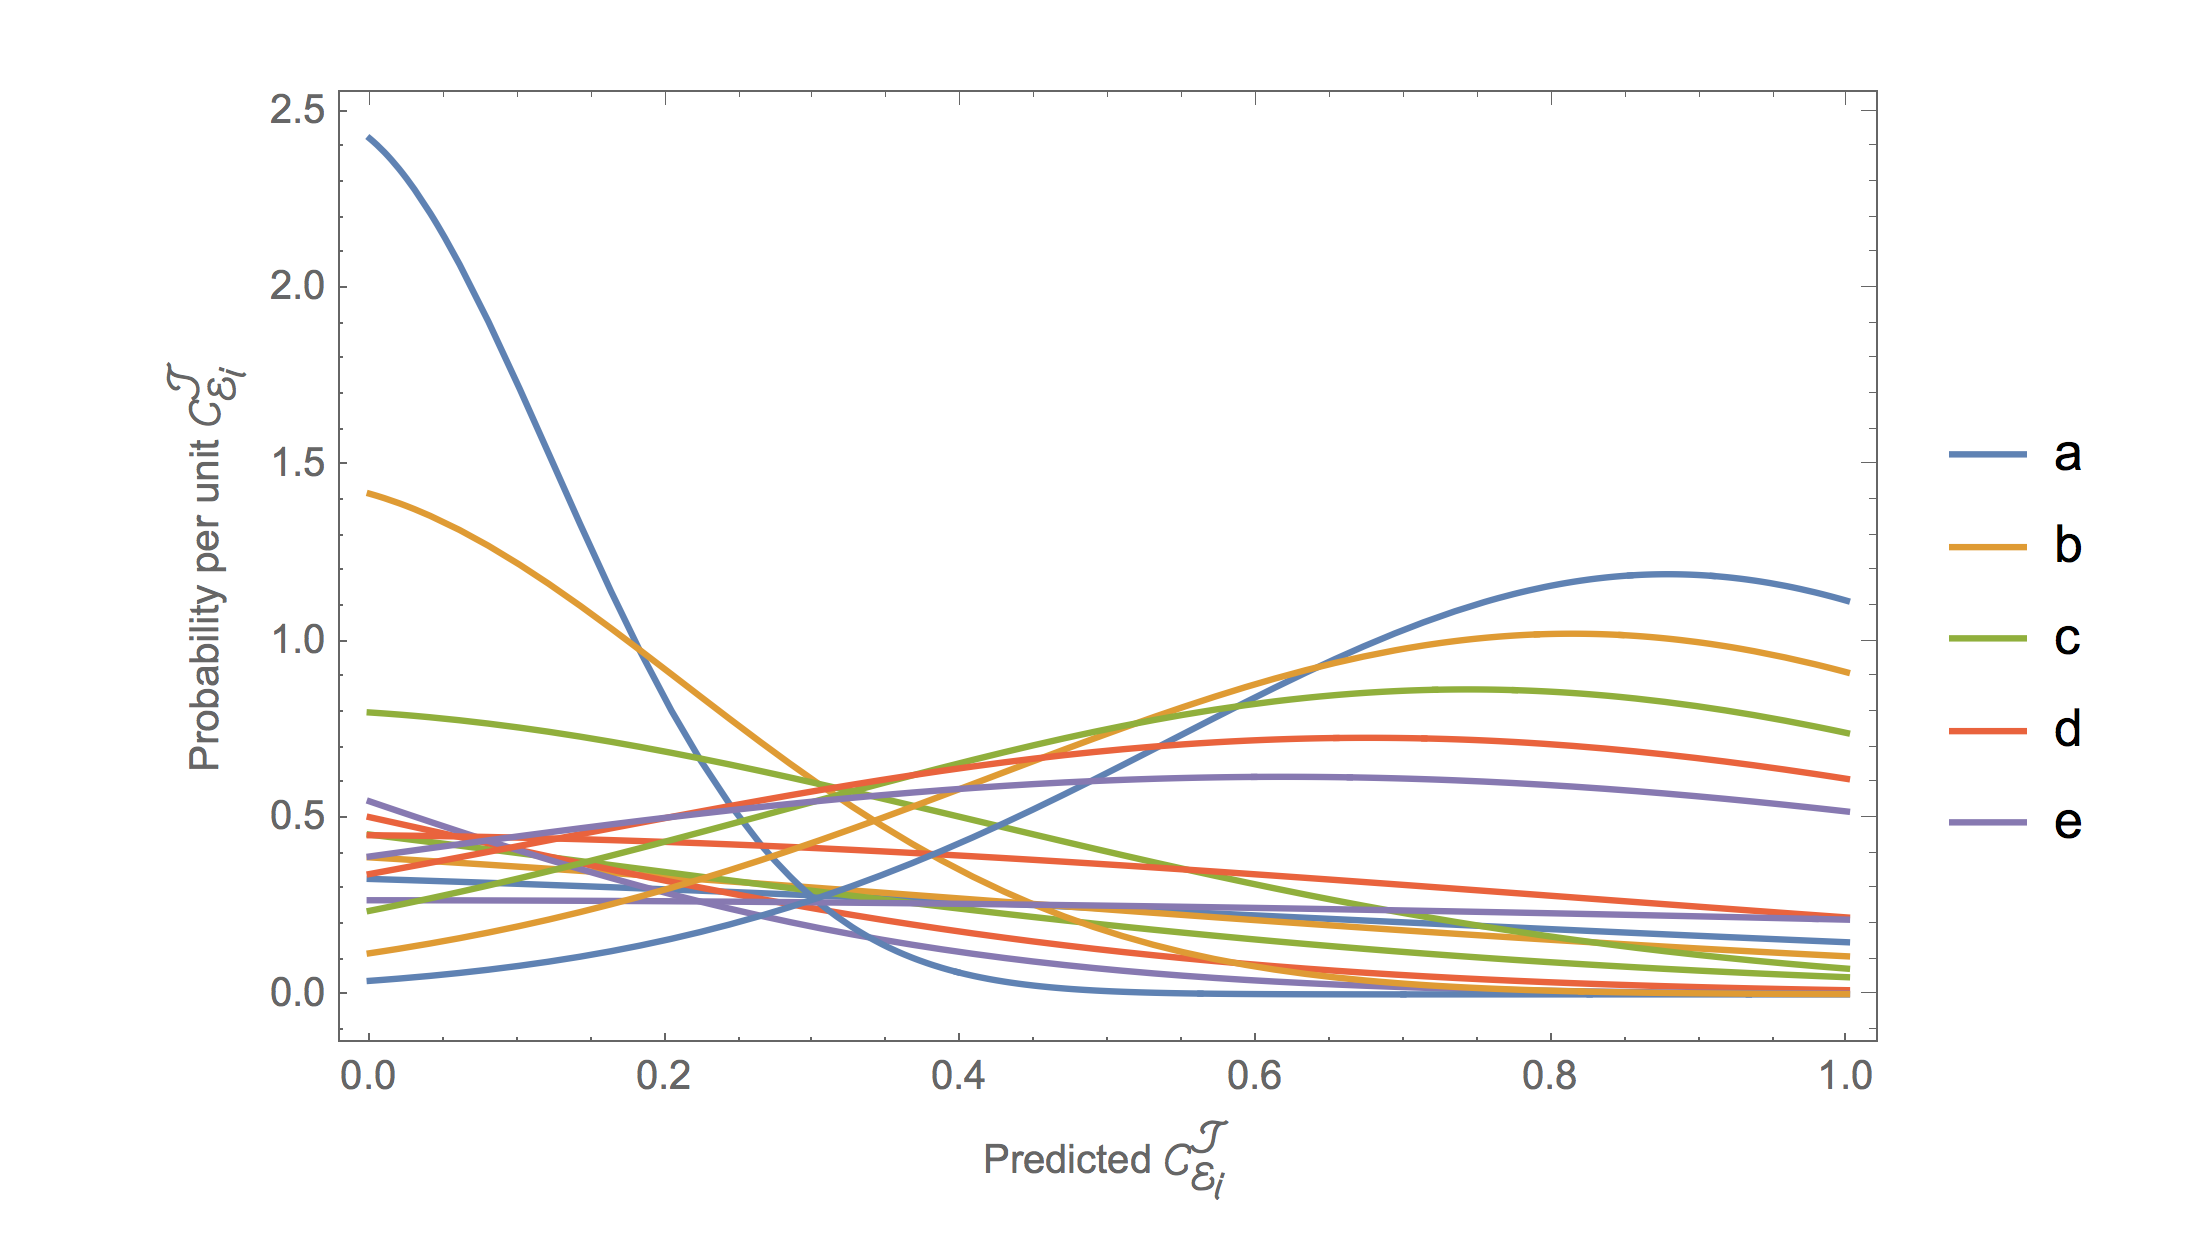
\includegraphics[width=1\textwidth]{figs/PredConf.png}
\centering
\caption{Probability density functions of estimates on flux control co\"efficients. Predictions were made at six disequilibrium ratio values, from three respective Mathematica neural network predictor functions, as referred to in \ref{chp:3}. The chosen disequilibrium ratios were $a = 0.01$, $b = 0.25$, $c = 0.50$, $d = 0.75$, and $e = 0.99$.}
\label{PredictionConfidence}
\end{figure}

Four hypothesis were set in order to further evaluate the gathered data. Based on the premise of covering all possible combinations of variables the first of these postulate that; at small disequilibrium ratios (far from equilibrium), large flux control co\"efficients are witnessed.

\begin{equation}\label{hyp1}
    \rho \ll 1 \Longrightarrow C_{E_i}^J \gg 0
\end{equation}

The second is derived from the reciprocal supposition, whereby large flux control co\"efficients necessitates small disequilibrium ratios.

\begin{equation}\label{hyp2}
    C_{E_i}^J \gg 0 \Longrightarrow \rho \ll 1
\end{equation}

With the first two hypothesis relating distances far from equilibrium to control, the third and forth relates to the opposite. With disequilibrium ratios approaching unity, the third hypothesis necessitates a small observed flux control co\"efficient.

\begin{equation}\label{hyp3}
    \rho \approx 1 \Longrightarrow C_{E_i}^J \ll 1
\end{equation}

While the final hypothesis views disequilibrium ratios as necessarily approaching unity where small flux control co\"efficients are concerned.

\begin{equation}\label{hyp4}
    C_{E_i}^J \ll 1 \Longrightarrow \rho \approx 1
\end{equation}

By testing these four hypothesis against the probability density function obtained from the data, one can gain insights into how thermodynamic states relate to own control behaviour. From figure \ref{TwoResPDF} it is clear that equations \ref{hyp1}, \ref{hyp2} and \ref{hyp3} holds true for most general cases. Equation \ref{hyp4} however holds the discrepancy as reactions with small disequilibrium ratios, as well as small flux control co\"efficients are observed. From the higher resolution figure \ref{TwoResPDF} $b$, outli\"ers can be seen in reactions closer to equilibrium, yet containing large degrees of flux control co\"efficients.

As of yet no further investigations have been undertaken into these specific outli\"ers and therefore no conclusions on them can be made. A hypothesis however, relates to the fact that reaction networks might exist in entirety at a distance close to equilirbium. In which case specific reactions will still maintain the larger degrees of flux control co\"efficients.




